\documentclass{ximera}

%\usepackage{todonotes}

\newcommand{\todo}{}

\usepackage{esint} % for \oiint
\ifxake%%https://math.meta.stackexchange.com/questions/9973/how-do-you-render-a-closed-surface-double-integral
\renewcommand{\oiint}{{\large\bigcirc}\kern-1.56em\iint}
\fi


\graphicspath{
  {./}
  {ximeraTutorial/}
  {basicPhilosophy/}
  {functionsOfSeveralVariables/}
  {normalVectors/}
  {lagrangeMultipliers/}
  {vectorFields/}
  {greensTheorem/}
  {shapeOfThingsToCome/}
  {dotProducts/}
  {partialDerivativesAndTheGradientVector/}
  {../productAndQuotientRules/exercises/}
  {../normalVectors/exercisesParametricPlots/}
  {../continuityOfFunctionsOfSeveralVariables/exercises/}
  {../partialDerivativesAndTheGradientVector/exercises/}
  {../directionalDerivativeAndChainRule/exercises/}
  {../commonCoordinates/exercisesCylindricalCoordinates/}
  {../commonCoordinates/exercisesSphericalCoordinates/}
  {../greensTheorem/exercisesCurlAndLineIntegrals/}
  {../greensTheorem/exercisesDivergenceAndLineIntegrals/}
  {../shapeOfThingsToCome/exercisesDivergenceTheorem/}
  {../greensTheorem/}
  {../shapeOfThingsToCome/}
  {../separableDifferentialEquations/exercises/}
  {vectorFields/}
}

\newcommand{\mooculus}{\textsf{\textbf{MOOC}\textnormal{\textsf{ULUS}}}}

\usepackage{tkz-euclide}
\usepackage{tikz}
\usepackage{tikz-cd}
\usetikzlibrary{arrows}
\tikzset{>=stealth,commutative diagrams/.cd,
  arrow style=tikz,diagrams={>=stealth}} %% cool arrow head
\tikzset{shorten <>/.style={ shorten >=#1, shorten <=#1 } } %% allows shorter vectors

\usetikzlibrary{backgrounds} %% for boxes around graphs
\usetikzlibrary{shapes,positioning}  %% Clouds and stars
\usetikzlibrary{matrix} %% for matrix
\usepgfplotslibrary{polar} %% for polar plots
\usepgfplotslibrary{fillbetween} %% to shade area between curves in TikZ
%\usetkzobj{all}
\usepackage[makeroom]{cancel} %% for strike outs
%\usepackage{mathtools} %% for pretty underbrace % Breaks Ximera
%\usepackage{multicol}
\usepackage{pgffor} %% required for integral for loops



%% http://tex.stackexchange.com/questions/66490/drawing-a-tikz-arc-specifying-the-center
%% Draws beach ball
\tikzset{pics/carc/.style args={#1:#2:#3}{code={\draw[pic actions] (#1:#3) arc(#1:#2:#3);}}}



\usepackage{array}
\setlength{\extrarowheight}{+.1cm}
\newdimen\digitwidth
\settowidth\digitwidth{9}
\def\divrule#1#2{
\noalign{\moveright#1\digitwidth
\vbox{\hrule width#2\digitwidth}}}




% \newcommand{\RR}{\mathbb R}
% \newcommand{\R}{\mathbb R}
% \newcommand{\N}{\mathbb N}
% \newcommand{\Z}{\mathbb Z}

\newcommand{\sagemath}{\textsf{SageMath}}


%\renewcommand{\d}{\,d\!}
%\renewcommand{\d}{\mathop{}\!d}
%\newcommand{\dd}[2][]{\frac{\d #1}{\d #2}}
%\newcommand{\pp}[2][]{\frac{\partial #1}{\partial #2}}
% \renewcommand{\l}{\ell}
%\newcommand{\ddx}{\frac{d}{\d x}}

% \newcommand{\zeroOverZero}{\ensuremath{\boldsymbol{\tfrac{0}{0}}}}
%\newcommand{\inftyOverInfty}{\ensuremath{\boldsymbol{\tfrac{\infty}{\infty}}}}
%\newcommand{\zeroOverInfty}{\ensuremath{\boldsymbol{\tfrac{0}{\infty}}}}
%\newcommand{\zeroTimesInfty}{\ensuremath{\small\boldsymbol{0\cdot \infty}}}
%\newcommand{\inftyMinusInfty}{\ensuremath{\small\boldsymbol{\infty - \infty}}}
%\newcommand{\oneToInfty}{\ensuremath{\boldsymbol{1^\infty}}}
%\newcommand{\zeroToZero}{\ensuremath{\boldsymbol{0^0}}}
%\newcommand{\inftyToZero}{\ensuremath{\boldsymbol{\infty^0}}}



% \newcommand{\numOverZero}{\ensuremath{\boldsymbol{\tfrac{\#}{0}}}}
% \newcommand{\dfn}{\textbf}
% \newcommand{\unit}{\,\mathrm}
% \newcommand{\unit}{\mathop{}\!\mathrm}
% \newcommand{\eval}[1]{\bigg[ #1 \bigg]}
% \newcommand{\seq}[1]{\left( #1 \right)}
% \renewcommand{\epsilon}{\varepsilon}
% \renewcommand{\phi}{\varphi}


% \renewcommand{\iff}{\Leftrightarrow}

% \DeclareMathOperator{\arccot}{arccot}
% \DeclareMathOperator{\arcsec}{arcsec}
% \DeclareMathOperator{\arccsc}{arccsc}
% \DeclareMathOperator{\si}{Si}
% \DeclareMathOperator{\scal}{scal}
% \DeclareMathOperator{\sign}{sign}


%% \newcommand{\tightoverset}[2]{% for arrow vec
%%   \mathop{#2}\limits^{\vbox to -.5ex{\kern-0.75ex\hbox{$#1$}\vss}}}
% \newcommand{\arrowvec}[1]{{\overset{\rightharpoonup}{#1}}}
% \renewcommand{\vec}[1]{\arrowvec{\mathbf{#1}}}
% \renewcommand{\vec}[1]{{\overset{\boldsymbol{\rightharpoonup}}{\mathbf{#1}}}}

% \newcommand{\point}[1]{\left(#1\right)} %this allows \vector{ to be changed to \vector{ with a quick find and replace
% \newcommand{\pt}[1]{\mathbf{#1}} %this allows \vec{ to be changed to \vec{ with a quick find and replace
% \newcommand{\Lim}[2]{\lim_{\point{#1} \to \point{#2}}} %Bart, I changed this to point since I want to use it.  It runs through both of the exercise and exerciseE files in limits section, which is why it was in each document to start with.

% \DeclareMathOperator{\proj}{\mathbf{proj}}
% \newcommand{\veci}{{\boldsymbol{\hat{\imath}}}}
% \newcommand{\vecj}{{\boldsymbol{\hat{\jmath}}}}
% \newcommand{\veck}{{\boldsymbol{\hat{k}}}}
% \newcommand{\vecl}{\vec{\boldsymbol{\l}}}
% \newcommand{\uvec}[1]{\mathbf{\hat{#1}}}
% \newcommand{\utan}{\mathbf{\hat{t}}}
% \newcommand{\unormal}{\mathbf{\hat{n}}}
% \newcommand{\ubinormal}{\mathbf{\hat{b}}}

% \newcommand{\dotp}{\bullet}
% \newcommand{\cross}{\boldsymbol\times}
% \newcommand{\grad}{\boldsymbol\nabla}
% \newcommand{\divergence}{\grad\dotp}
% \newcommand{\curl}{\grad\cross}
%\DeclareMathOperator{\divergence}{divergence}
%\DeclareMathOperator{\curl}[1]{\grad\cross #1}
% \newcommand{\lto}{\mathop{\longrightarrow\,}\limits}

% \renewcommand{\bar}{\overline}

\colorlet{textColor}{black}
\colorlet{background}{white}
\colorlet{penColor}{blue!50!black} % Color of a curve in a plot
\colorlet{penColor2}{red!50!black}% Color of a curve in a plot
\colorlet{penColor3}{red!50!blue} % Color of a curve in a plot
\colorlet{penColor4}{green!50!black} % Color of a curve in a plot
\colorlet{penColor5}{orange!80!black} % Color of a curve in a plot
\colorlet{penColor6}{yellow!70!black} % Color of a curve in a plot
\colorlet{fill1}{penColor!20} % Color of fill in a plot
\colorlet{fill2}{penColor2!20} % Color of fill in a plot
\colorlet{fillp}{fill1} % Color of positive area
\colorlet{filln}{penColor2!20} % Color of negative area
\colorlet{fill3}{penColor3!20} % Fill
\colorlet{fill4}{penColor4!20} % Fill
\colorlet{fill5}{penColor5!20} % Fill
\colorlet{gridColor}{gray!50} % Color of grid in a plot

\newcommand{\surfaceColor}{violet}
\newcommand{\surfaceColorTwo}{redyellow}
\newcommand{\sliceColor}{greenyellow}




\pgfmathdeclarefunction{gauss}{2}{% gives gaussian
  \pgfmathparse{1/(#2*sqrt(2*pi))*exp(-((x-#1)^2)/(2*#2^2))}%
}


%%%%%%%%%%%%%
%% Vectors
%%%%%%%%%%%%%

%% Simple horiz vectors
\renewcommand{\vector}[1]{\left\langle #1\right\rangle}


%% %% Complex Horiz Vectors with angle brackets
%% \makeatletter
%% \renewcommand{\vector}[2][ , ]{\left\langle%
%%   \def\nextitem{\def\nextitem{#1}}%
%%   \@for \el:=#2\do{\nextitem\el}\right\rangle%
%% }
%% \makeatother

%% %% Vertical Vectors
%% \def\vector#1{\begin{bmatrix}\vecListA#1,,\end{bmatrix}}
%% \def\vecListA#1,{\if,#1,\else #1\cr \expandafter \vecListA \fi}

%%%%%%%%%%%%%
%% End of vectors
%%%%%%%%%%%%%

%\newcommand{\fullwidth}{}
%\newcommand{\normalwidth}{}



%% makes a snazzy t-chart for evaluating functions
%\newenvironment{tchart}{\rowcolors{2}{}{background!90!textColor}\array}{\endarray}

%%This is to help with formatting on future title pages.
\newenvironment{sectionOutcomes}{}{}



%% Flowchart stuff
%\tikzstyle{startstop} = [rectangle, rounded corners, minimum width=3cm, minimum height=1cm,text centered, draw=black]
%\tikzstyle{question} = [rectangle, minimum width=3cm, minimum height=1cm, text centered, draw=black]
%\tikzstyle{decision} = [trapezium, trapezium left angle=70, trapezium right angle=110, minimum width=3cm, minimum height=1cm, text centered, draw=black]
%\tikzstyle{question} = [rectangle, rounded corners, minimum width=3cm, minimum height=1cm,text centered, draw=black]
%\tikzstyle{process} = [rectangle, minimum width=3cm, minimum height=1cm, text centered, draw=black]
%\tikzstyle{decision} = [trapezium, trapezium left angle=70, trapezium right angle=110, minimum width=3cm, minimum height=1cm, text centered, draw=black]


\title{Encoding Visually}


\begin{document}

\begin{abstract}
pairs to dots
\end{abstract}
\maketitle


Function notation allows us to talk about individual pairs inside a function.


\begin{center}
\textbf{\textcolor{purple!85!blue}{(d, F(d))}}
\end{center}




$d$ is sitting in the left position of our ordered pair, therefore it represents a domain number. $F(d)$ represents the value of the function at $d$ and is written on the right in the ordered pair.


\begin{example} Ordered Pairs

Suppose $4$ is a member of the domain of the function $H$. \\
Then $H(4)$ represents the value of $H$ at $4$. \\
$H(4)$ is a member of the range of $H$. \\
$(4, H(4))$ is a pair in the function $H$.

If we happen to know that $(4, 9)$ is a pair in the function $H$, then we know $H(4) = \answer{9}$.

\end{example}
The equation in the example is just communicating that the expressions $H(4)$ and $9$ represent the same value in this situation. \\

That was looking at the function $H$ one pair at a time. \\



In addition to talking about individual pairs, we might also like to talk about the whole collection at once.  Our first attempt at this is via pictures. We need a way to visually represent a single pair and then convert all pairs to a picture.  With this picture, we can analyze the function as a whole, identify important places in the domain, detect trends in the data, and quickly estimate information about the whole function.














\section*{Visually Encoding}

Let $f$ be a function and $d$ a domain number of $f$. \\

Our plan is to visually encode the pair $(d,f(d))$ as a dot in the Cartesian plane with coordinates $(d,f(d))$.

\begin{center}
\large{\textbf{\textcolor{red!90!darkgray}{That's It!}}}  
\end{center}








\begin{image}
\begin{tikzpicture}
        \begin{axis}[
            domain=0:4, ymax=5, xmax=5, ymin=-5, xmin=-5,
            axis lines =center, xlabel=$domain$, ylabel=$codomain$,
            ticklabel style={font=\scriptsize},
            every axis y label/.style={at=(current axis.above origin),anchor=south},
            every axis x label/.style={at=(current axis.right of origin),anchor=west},
            axis on top
          ]
          
        \addplot [color=penColor2,only marks,mark=*] coordinates{(3,2)};


        \draw[decoration={brace,raise=.2cm,mirror},decorate,thin] (axis cs:3.05,0)--(axis cs:3.05,2);
        \draw[decoration={brace,raise=.2cm},decorate,thin] (axis cs:0,2.05)--(axis cs:3,2.05);
        \node[anchor=east] at (axis cs:1.85,3) {$d$};
        \node[anchor=east] at (axis cs:4.7,1) {$f(d)$};
                     
        \node at (axis cs:4,2.7) [penColor] {$(d,f(d))$};

        \end{axis}
\end{tikzpicture}
\end{image}







\textbf{\textcolor{blue!55!black}{$\blacktriangleright$ desmos graph}} 
\begin{center}
\desmos{bhllb4u1ng}{400}{300}
\end{center}
\end{example}





From the origin, we measure horizontally a distance of $d$.  Then we measure a vertical distance of $f(d)$. Plot a dot. The horizontal and vertical measurements for a point are called its \textit{coordinates}.


\begin{itemize}
\item The horizontal coordinate is the domain number.
\item The vertical coordinate is the function value.
\end{itemize}





\begin{explanation} \textbf{Video: Visually Encoding Function Pairs}

[ Click on the arrow to the right to expand the video. ]
\begin{expandable} 

\begin{center}
\youtube{PRBmHmutSAY}
\end{center}

\end{expandable}
\end{explanation}










\begin{example}

Suppose we have a function $M$ and we know that $M(3)=2$. This information can be encoded visually with a dot plotted at $(3, 2)$.

\begin{image}
\begin{tikzpicture}
\begin{axis}[
            domain=0:4, ymax=5, xmax=5, ymin=-5, xmin=-5,
            axis lines =center, xlabel=$domain$, ylabel=$codomain$,
            ticklabel style={font=\scriptsize},
            every axis y label/.style={at=(current axis.above origin),anchor=south},
            every axis x label/.style={at=(current axis.right of origin),anchor=west},
            axis on top
          ]
        
          \addplot [color=penColor2,only marks,mark=*] coordinates{(3,2)};


          \draw[decoration={brace,raise=.2cm,mirror},decorate,thin] (axis cs:3.05,0)--(axis cs:3.05,2);
          \draw[decoration={brace,raise=.2cm},decorate,thin] (axis cs:0,2.05)--(axis cs:3,2.05);
          \node[anchor=east] at (axis cs:1.85,3) {$3$};
          \node[anchor=east] at (axis cs:4,1) {$2$};
                    
          
          \node at (axis cs:3.7,2.7) [penColor] {$(3,2)$};

        \end{axis}
\end{tikzpicture}
\end{image}





\textbf{\textcolor{blue!55!black}{$\blacktriangleright$ desmos graph}} 
\begin{center}
\desmos{ckcwkruxgv}{400}{300}
\end{center}
\end{example}



\begin{question}
Suppose we have a graph of $y=H(t)$ and one of the following four points is on this graph. Which point would be on the graph if $H(-3) = -2$?
\begin{image}
\begin{tikzpicture}
\begin{axis}[
            domain=0:4, ymax=5, xmax=5, ymin=-5, xmin=-5,
            axis lines =center, xlabel=$t$, ylabel=$y$,
            ticklabel style={font=\scriptsize},
            every axis y label/.style={at=(current axis.above origin),anchor=south},
            every axis x label/.style={at=(current axis.right of origin),anchor=west},
            axis on top
          ]

          
        \addplot [color=penColor2,only marks,mark=*] coordinates{(-3,2)};
        \addplot [color=penColor2,only marks,mark=*] coordinates{(3,-2)};
        \addplot [color=penColor2,only marks,mark=*] coordinates{(-3,-2)};
        \addplot [color=penColor2,only marks,mark=*] coordinates{(3,2)};

        \node at (axis cs:-3.4,2.4) [penColor] {$A$};
        \node at (axis cs:3.4,2.4) [penColor] {$B$};
        \node at (axis cs:-3.4,-2.4) [penColor] {$C$};
        \node at (axis cs:3.4,-2.4) [penColor] {$D$};

\end{axis}
\end{tikzpicture}
\end{image}






\textbf{\textcolor{blue!55!black}{$\blacktriangleright$ desmos graph}} 
\begin{center}
\desmos{gnwxm58g3s}{400}{300}
\end{center}
\end{example}






\begin{multipleChoice}
\choice {$A$}
\choice {$B$}
\choice[correct] {$C$}
\choice {$D$}
\end{multipleChoice}


\textbf{Note: } The horizontal axis is named $t$, because the function notation, $H(t)$, tells us that $t$ represents the domain numbers.  We generally name the vertical axis with some name not already in use, like $y$.  Then, we let the reader know that the values of $y$ are representing values of the function, $y=H(t)$.
\end{question}



\begin{question}
Suppose $k$ is a function with $k(-1)>0$. When we consider the graph of $y=k(t)$, there will be a point corresponding to $k(-1)$. In which quadrant will the corresponding dot be plotted?
\begin{image}
\begin{tikzpicture}
\begin{axis}[
            domain=0:4, ymax=5, xmax=5, ymin=-5, xmin=-5,
            axis lines =center, xlabel=$t$, ylabel=$y$,
            ticklabel style={font=\scriptsize},
            every axis y label/.style={at=(current axis.above origin),anchor=south},
            every axis x label/.style={at=(current axis.right of origin),anchor=west},
            axis on top
          ]

        
        \node at (axis cs:3.4,2.4) [penColor] {$I$};
        \node at (axis cs:-3.4,2.4) [penColor] {$II$};
        \node at (axis cs:-3.4,-2.4) [penColor] {$III$};
        \node at (axis cs:3.4,-2.4) [penColor] {$IV$};

\end{axis}
\end{tikzpicture}
\end{image}


\textbf{\textcolor{blue!55!black}{$\blacktriangleright$ desmos graph}} 
\begin{center}
\desmos{19uamtbsyp}{400}{300}
\end{center}



\begin{multipleChoice}
\choice {$I$}
\choice[correct] {$II$}
\choice {$II$}
\choice {$IV$}
\end{multipleChoice}

\end{question}
Four quadrants for the four possible combinations of domain and codomain signs. \\


A graph of a function is just a collection of a bunch of dots.  Each dot represents a pair in the function.  Each dot has two coordinates.  The horizontal (first/left) coordinate is the domain number and the vertical (second/right) coordinate is the function value at that domain value.

The functions we are most interested in have millions of billions of trillions of dots.  



\begin{image}
\begin{tikzpicture} 
  \begin{axis}[
            domain=-4:4, ymax=5, xmax=4, ymin=-5, xmin=-4,
            axis lines =center, xlabel=$t$, ylabel={$y=g(t)$},
            ticklabel style={font=\scriptsize},
            every axis y label/.style={at=(current axis.above origin),anchor=south},
            every axis x label/.style={at=(current axis.right of origin),anchor=west},
            axis on top
          ]
          
    \addplot [color=penColor2,only marks,mark=*] coordinates{(-2,5) (-1,0) (0,-3) (1,-4) (2,-3) (3,0)};
           

  \end{axis}
\end{tikzpicture}
\end{image}




\textbf{\textcolor{blue!55!black}{$\blacktriangleright$ desmos graph}} 
\begin{center}
\desmos{jjso0hzpgp}{400}{300}
\end{center}




As we add more and more dots....


\begin{image}
\begin{tikzpicture} 
  \begin{axis}[
            domain=-4:4, ymax=5, xmax=4, ymin=-5, xmin=-4,
            axis lines =center, xlabel=$t$, ylabel={$y=g(t)$},
            ticklabel style={font=\scriptsize},
            every axis y label/.style={at=(current axis.above origin),anchor=south},
            every axis x label/.style={at=(current axis.right of origin),anchor=west},
            axis on top
          ]
          
    \addplot [color=penColor2,only marks,mark=*] coordinates{(-2.5,8.25) (-2,5) (-1.5,2.25) (-1,0) (-0.5,-1.75) (0,-3) (0.5,-3.75) (1,-4) (1.5,-3.75) (2,-3) (2.5,-1.75) (3,0) (3.5,2.25)};
           

  \end{axis}
\end{tikzpicture}
\end{image}


It soon becomes difficult to distinguish the individual dots.

\begin{image}
\begin{tikzpicture} 
  \begin{axis}[
            domain=-4:4, ymax=5, xmax=4, ymin=-5, xmin=-4,
            axis lines =center, xlabel=$t$, ylabel={$y=g(t)$},
            ticklabel style={font=\scriptsize},
            every axis y label/.style={at=(current axis.above origin),anchor=south},
            every axis x label/.style={at=(current axis.right of origin),anchor=west},
            axis on top
          ]
          
      \foreach \x in {-3,-2.75,...,3}
      \addplot [color=penColor2,only marks,mark=*] coordinates{(\x,\x*\x-2*\x-3)};
           

  \end{axis}
\end{tikzpicture}
\end{image}


They begin to overlap...

\begin{image}
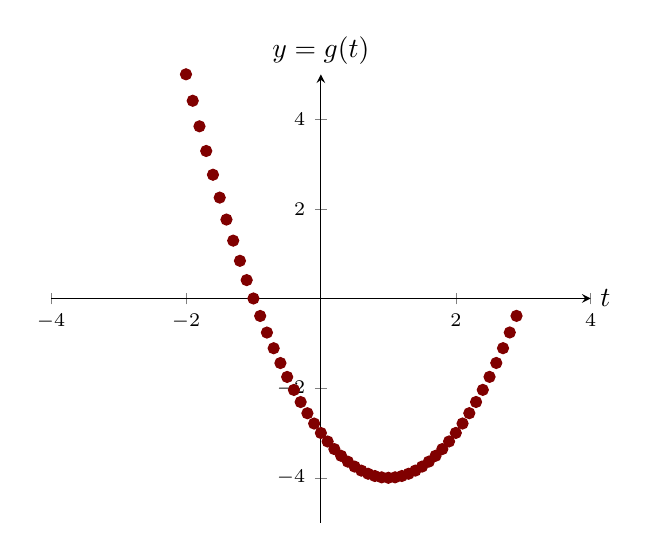
\begin{tikzpicture} 
  \begin{axis}[
            domain=-4:4, ymax=5, xmax=4, ymin=-5, xmin=-4,
            axis lines =center, xlabel=$t$, ylabel={$y=g(t)$},
            ticklabel style={font=\scriptsize},
            every axis y label/.style={at=(current axis.above origin),anchor=south},
            every axis x label/.style={at=(current axis.right of origin),anchor=west},
            axis on top
          ]
          
      \foreach \x in {-3,-2.9,...,3}
      \addplot [color=penColor2,only marks,mark=*] coordinates{(\x,\x*\x-2*\x-3)};
           

  \end{axis}
\end{tikzpicture}
\end{image}




Eventually, your eyes play tricks on you.  You think you see a single object.  A thing - like a wire bent on a piece of paper.



\begin{image}
\begin{tikzpicture} 
  \begin{axis}[
            domain=-4:4, ymax=5, xmax=4, ymin=-5, xmin=-4,
            axis lines =center, xlabel=$t$, ylabel={$y=g(t)$},
            ticklabel style={font=\scriptsize},
            every axis y label/.style={at=(current axis.above origin),anchor=south},
            every axis x label/.style={at=(current axis.right of origin),anchor=west},
            axis on top
          ]
          
    \addplot [draw=penColor2,very thick,smooth] {(x+1)*(x-3)};
           

  \end{axis}
\end{tikzpicture}
\end{image}



\large{It isn't!!!!}




It is a bunch of individual dots very close together. They are forming a pattern that your eye likes. Your eye glues them together.  Much of this course is about these eye-pleasing patterns that functions create.





\begin{question}
Suppose the domain of the function, $p$, only contains positive numbers.  Which quadrants cannot contain points on the graph of $y=p(k)$?

\begin{selectAll}
\choice {$I$}
\choice[correct] {$II$}
\choice[correct] {$III$}
\choice {$IV$}
\end{selectAll}

\end{question}




















\section*{Dots}



Of course, the dots on a graph of a function are wrong. They are too big. Dots, even the size of a pencil point, cover millions of billions of points. If you doubt that, then look at the graph under a microscope.

Does the graph below tell us that $K(1) = -4$ or $K(1.03) = -4.1$ or $K(0.95) = -3.97$ or $K(1.01) = -3.95$?

\begin{image}
\begin{tikzpicture} 
  \begin{axis}[
            domain=-4:4, ymax=5, xmax=4, ymin=-5, xmin=-4,
            axis lines =center, xlabel=$v$, ylabel={$y=K(v)$},
            ticklabel style={font=\scriptsize},
            every axis y label/.style={at=(current axis.above origin),anchor=south},
            every axis x label/.style={at=(current axis.right of origin),anchor=west},
            axis on top
          ]
          
    \addplot [color=penColor2,only marks,mark=*] coordinates{(-2,5) (-1,0) (0,-3) (1,-4) (2,-3) (3,0)};
           

  \end{axis}
\end{tikzpicture}
\end{image}

The answer is yes.  \\


It says all of those, because the dots are too big.  Our graph should consist of points, but points are dimensionless.  We wouldn't be able to see them.  So, we draw dots that we can see and accept the inaccuracy of the graph.

Therefore, graphs are inherently inaccurate and there is nothing you can do about that.  Graphs are communication tools. We have to keep this in mind when discussing mathematics with other people. Algebra is our tool for exactness.  Graphs give us the overall picture, but at the expense of accuracy.

We want to use both Algebra and graphs.  They each tell us what the other should be doing.  We just have to remember what each tool provides us.






\begin{explanation} \textbf{Video: Graphs are Inherently Inaccurate}

[ Click on the arrow to the right to expand the video. ]
\begin{expandable} 

\begin{center}
\youtube{0KOR07LdC8A}
\end{center}

\end{expandable}
\end{explanation}














\section*{Domain and Range}


From our visual encoding plan, we see that the first coordinate of each dot will be a number from the domain of the function and the second coordinate of each dot will be a number from the range of the function.  More specifically, the second coordinate is the function value at the first coordinate.  The horizontal and vertical axis are seen as holding the domain and range.

\begin{itemize}
\item \textbf{DOMAIN:} We think of the domain as sitting on the horizontal axis.
\item \textbf{RANGE:} We think of the range as sitting on the vertical axis.
\end{itemize}


The two axes in our Cartesian plane are performing double duty.  We need double vision to see them correctly. If a dot on the graph happens to land on an axis, then we have function value information.

If the graph of $y=K(v)$ included three dots on the axes...

\begin{image}
\begin{tikzpicture} 
  \begin{axis}[
            domain=-4:4, ymax=5, xmax=4, ymin=-5, xmin=-4,
            axis lines =center, xlabel=$v$, ylabel={$y=K(v)$},
            ticklabel style={font=\scriptsize},
            every axis y label/.style={at=(current axis.above origin),anchor=south},
            every axis x label/.style={at=(current axis.right of origin),anchor=west},
            axis on top
          ]
          
    \addplot [color=penColor2,only marks,mark=*] coordinates{(-2,5) (-1,0) (0,-3) (1,-4) (2,-3) (3,0)};
           

  \end{axis}
\end{tikzpicture}
\end{image}


... on one hand...
\begin{itemize}
\item The dot at $(-1,0)$ tells us that $K(-1) = 0$.
\item The dot at $(0,-3)$ tells us that $K(0) = -3$.
\item The dot at $(3,0)$ tells us that $K(3) = 0$.
\end{itemize}


...on the other hand, from all of the dots, we can see that the domain of $K$ includes $\{ -2, -1, 0, 1, 2, 3 \}$.  This is the collection of all of the first coordinates of all of the dots.


What if we want to visualize the domain and the range of the function, by themselves?  When visualizing the domain and range, we would view each axes as an individual number line.  Rather than thinking of the axes as holding dots with two coordinates, we would think that the axes are number lines, holding numbers, and we would color in the intervals and numbers, like on a number line.

We need our brains to jump back and forth between these views.  Dots represent pairs in a function.  We decipher these pairs of numbers by the location of the dot.  At the same time, locations on the axes also represent domain and range numbers - depending on the plotted dots.





\begin{explanation} \textbf{Video: Double Duty}

[ Click on the arrow to the right to expand the video. ]
\begin{expandable} 

\begin{center}
\youtube{X0nD5I5D6fI}
\end{center}

\end{expandable}
\end{explanation}








\begin{example} 


Below is the graph of $y=h(f)$. We can identify its domain, by collecting all of the first coordinates of all of the dots.   We can identify its range, by collecting all of the second coordinates of all of the dots.  


\begin{image}
\begin{tikzpicture} 
  \begin{axis}[
            domain=-10:10, ymax=10, xmax=10, ymin=-10, xmin=-10,
            axis lines =center, xlabel=$f$, ylabel={$y=h(f)$},
            ticklabel style={font=\scriptsize},
            every axis y label/.style={at=(current axis.above origin),anchor=south},
            every axis x label/.style={at=(current axis.right of origin),anchor=west},
            axis on top
          ]
          
          \addplot [line width=2, penColor, smooth,samples=100,domain=(-4:0)] ({x},{-0.5*x+1});
          \addplot [line width=2, penColor, smooth,samples=100,domain=(1:7)] ({x},{0.5*x-7});
          \addplot [color=penColor,only marks,mark=*] coordinates{(-4,3) (0,1) (7,-3.5)};
          \addplot [color=penColor,fill=white,only marks,mark=*] coordinates{(1,-6.5)};


  \end{axis}
\end{tikzpicture}
\end{image}


\begin{explanation}
We could think of the horizontal axis as the domain number line, squeeze all of the dots to the horizontal axis, and draw in the intervals of the domain.
\[
domain = [-4,0] \cup (1,7]
\]

\begin{image}
\begin{tikzpicture} 
  \begin{axis}[
            domain=-10:10, ymax=10, xmax=10, ymin=-10, xmin=-10,
            axis lines =center, xlabel=$f$, ylabel={$y=h(f)$},
            ticklabel style={font=\scriptsize},
            every axis y label/.style={at=(current axis.above origin),anchor=south},
            every axis x label/.style={at=(current axis.right of origin),anchor=west},
            axis on top
          ]
          
          \addplot [line width=2, penColor, smooth,samples=100,domain=(-4:0)] ({x},{-0.5*x+1});
          \addplot [line width=2, penColor, smooth,samples=100,domain=(1:7)] ({x},{0.5*x-7});
          \addplot [color=penColor,only marks,mark=*] coordinates{(-4,3) (0,1) (7,-3.5)};
          \addplot [color=penColor,fill=white,only marks,mark=*] coordinates{(1,-6.5)};


          \addplot [line width=2, penColor2, smooth,samples=100,domain=(-4:0)] ({x},{0});
          \addplot [line width=2, penColor2, smooth,samples=100,domain=(1:7)] ({x},{0});
          \addplot [color=penColor2,only marks,mark=*] coordinates{(-4,0) (0,0) (7,0)};
          \addplot [color=penColor2,fill=white,only marks,mark=*] coordinates{(1,0)};
           

  \end{axis}
\end{tikzpicture}
\end{image}



We could think of the vertical axis as the range number line, squeeze all of the points to the vertical axis, and draw in the intervals of the range.

\[
range = (-6.5, -3.5] \cup [1, 4]
\]

\begin{image}
\begin{tikzpicture} 
  \begin{axis}[
            domain=-10:10, ymax=10, xmax=10, ymin=-10, xmin=-10,
            axis lines =center, xlabel=$f$, ylabel={$y=h(f)$},
            ticklabel style={font=\scriptsize},
            every axis y label/.style={at=(current axis.above origin),anchor=south},
            every axis x label/.style={at=(current axis.right of origin),anchor=west},
            axis on top
          ]
          
          \addplot [line width=2, penColor, smooth,samples=100,domain=(-4:0)] ({x},{-0.5*x+1});
          \addplot [line width=2, penColor, smooth,samples=100,domain=(1:7)] ({x},{0.5*x-7});
          \addplot [color=penColor,only marks,mark=*] coordinates{(-4,3) (0,1) (7,-3.5)};
          \addplot [color=penColor,fill=white,only marks,mark=*] coordinates{(1,-6.5)};

          \addplot [line width=2, penColor2, smooth,samples=100,domain=(-6.5:-3.5)] ({0},{x});
          \addplot [line width=2, penColor2, smooth,samples=100,domain=(1:4)] ({0},{x});
          \addplot [color=penColor2,only marks,mark=*] coordinates{(0,-3.5) (0,1) (0,4)};
           \addplot [color=penColor2,fill=white,only marks,mark=*] coordinates{(0,-6.5)};
           

  \end{axis}
\end{tikzpicture}
\end{image}

\end{explanation}
\end{example}



This presents a communication issue.  \\


When we were drawing intervals on numbers lines, we used square brackets and parentheses to signal the inclusion or exclusion of numbers.  Now we are using filled and hollow dots. \\

This is due to the long history of mathematics.  We must be ready to read and understand both.


\begin{itemize}
\item Filled (or closed) dots and square brackets indicate the inclusion of a number or a point.
\item Hollow (or open) dots and parentheses indicate the exclusion of a number or a point.
\end{itemize}

Unfortunately, the term \textbf{endpoint} is used for the end numbers of intervals, when really they are end-numbers. Again, more language we must be aware of.

In this course, we will try to deliberately and appropriately use number and point.  As you discuss mathematics with more people, you will encounter different usage.



\begin{example}

Below is the graph of $z=P(k)$.  Use it to answer the following questions.

\begin{image}
\begin{tikzpicture} 
  \begin{axis}[
            domain=-10:10, ymax=10, xmax=10, ymin=-10, xmin=-10,
            axis lines =center, xlabel=$k$, ylabel={$z=P(k)$},
            ticklabel style={font=\scriptsize},
            every axis y label/.style={at=(current axis.above origin),anchor=south},
            every axis x label/.style={at=(current axis.right of origin),anchor=west},
            axis on top
          ]
          
          \addplot [line width=2, penColor, smooth,samples=100,domain=(-5:0)] ({x},{(x+5)*(1-x)});
          \addplot [line width=2, penColor, smooth,samples=100,domain=(1:5)] ({x},{-x-1});

          \addplot [color=penColor,fill=white,only marks,mark=*] coordinates{(0,5) (1,-2)};
          \addplot [color=penColor,only marks,mark=*] coordinates{(-5,0) (5,-6)};


           

  \end{axis}
\end{tikzpicture}
\end{image}








\begin{question}

What is the domain of $P(k)$?

\begin{multipleChoice}
  \choice {$[-5,0] \cup [1,5]$}
  \choice {$[-5,5]$}
  \choice {$(-5,0] \cup [1,5)$}
  \choice [correct]{$[-5,0) \cup (1,5]$}
  \choice {$[-5,0), (1,5]$}
\end{multipleChoice}

\end{question}






\begin{question}

What is the range of $P(k)$?

\begin{multipleChoice}
  \choice {$[-6,9]$}
  \choice [correct]{$[-6,-2) \cup [0,9]$}
  \choice {$[-6,-2) \cup [0,5)$}
  \choice {$[-6,-2), [0,9]$}
\end{multipleChoice}

\end{question}






\end{example}













\begin{center}
\textbf{\textcolor{green!50!black}{ooooo-=-=-=-ooOoo-=-=-=-ooooo}} \\

more examples can be found by following this link\\ \link[More Examples of Function Graphs]{https://ximera.osu.edu/csccmathematics/precalculus1/precalculus1/functionGraphs/examples/exampleList}

\end{center}


\end{document}
